\documentclass[french]{article}
\usepackage[T1]{fontenc}
\usepackage[utf8]{inputenc}
\usepackage{lipsum}
\usepackage{lmodern}
\usepackage{geometry}
\usepackage{babel}
\usepackage{graphicx}
\usepackage{lastpage}
\usepackage{ragged2e}
\usepackage{enumitem}
\usepackage[normalem]{ulem}
\usepackage{hyperref} % pour \url{URL}
\usepackage{color} % pour \textcolor{color}{text}
\usepackage{listings} % pour afficher du code
\usepackage{longtable} % pour l'environnement longtable
\usepackage{float} % pour des figures non flottantes
\usepackage{amsmath}

% Grammaire EBNF
\usepackage{syntax}
\setlength{\grammarparsep}{5pt plus 1pt minus 1pt}
\setlength{\grammarindent}{11em}

<<<<<<< HEAD
% Diagramme de flux
\usepackage{tikz}
\usepackage{forest}
\usetikzlibrary{shapes,arrows,positioning,shadows,matrix}

% Matrices
\usepackage{kbordermatrix}% http://www.hss.caltech.edu/~kcb/TeX/kbordermatrix.sty
=======
% Dessin avec tikz
\usepackage{tikz} % figure en tout genre
\usepackage{forest} % arbre
\usetikzlibrary{shapes,arrows,positioning,shadows}
>>>>>>> 96f4cb76be9d7640a89b388fe049cbab975819a3

% Style C++
\lstset{
	language=C++,
	tabsize=2,
	basicstyle=\small\ttfamily,
	keywordstyle=\color{blue},
	stringstyle=\color{red},
	commentstyle=\color{black!40},
	morecomment=[l][\color{black!50}]{\#},
	gobble=10,
	frame=single,
	otherkeywords={constexpr,std,string,vector,map,pair,size\_t,function,remove\_const,remove\_reference}
}

\geometry{
	a4paper,
	total={210mm,297mm},
	left=20mm,
	right=20mm,
	top=20mm,
	bottom=20mm,
}

\usepackage{fancyhdr}
\pagestyle{fancy}
\setlist[enumerate,1]{leftmargin=2cm}

% Entêtes
\lhead{Browne Champion Djomo Hardy Richoz Rochat}
\chead{}
\rhead{PRO}
\renewcommand{\headrulewidth}{0.4pt}
\renewcommand{\footrulewidth}{0.4pt}

\begin{document}
	
	% Titre du document
	\title{GraphY} % ou un autre nom
	\author{Rapport\\ 
		Projet de semestre\\
		Browne Champion Djomo Hardy Richoz Rochat\\
		Resp. René Rentsch\\
		HEIG-VD}
	\date{\today} % date du jour
	\maketitle
	
	% Tables des matières
	\tableofcontents
	
	% Tables des figures
	\listoffigures
	
	% Pour tout le document
	\justify
	\normalsize
	
	\section{Cadre de développement} 
		L'application est développée à l'aide du langage C++ et de la bibliothèque Qt \textcolor{red}{(insérer les versions utilisées ainsi que les compilateurs ?)}. Afin que le code source soit écrit dans le même style par tous les membres du groupe, nous avons décidé d'utiliser le Coding Style de Qt \cite{qtStyle} qui correspond bien à nos besoins.
			
	\section{Interpréteur} % Champion
		Dans le cadre de l'application, l'utilisateur est amené à entrer des commandes lui permettant de créer et de modifier des graphes, tout autant que d'appeler des fonctions effectuant différents traitements (algorithmes, lecture depuis un fichier, ...). 
	
		\subsection{Normalisation du langage} 
			Il est nécessaire de définir une grammaire claire sur la syntaxe des commandes, ainsi que leur sémantique.
			
			\subsubsection{Analyse des types et des opérations} 
				Premièrement, il faut définir les types disponibles dans le langage. Pour cela, il est intéressant de partir des algorithmes de graphe et de voir les types de résultats que nous attendons en sortie, ainsi que les types de paramètres dont nous aurons besoin:
			
				\begin{itemize}
					\item Boolean: un graphe a-t-il un cycle? est-il eulérien? ...
					\item Number: poids d'un arc, indice d'un sommet, ...
					\begin{itemize}
						\item Integer: pour les index, ...
						\item Float: pour les poids, ...
					\end{itemize}
					\item String: label d'un sommet, nom d'une fonction, ...
					\item Array: liste d'arêtes, matrices (Floyd-Warshall), ...
					\item Graph: le graphe à proprement parler
					\begin{itemize}
						\item Vertex: un sommet, son indice, son poids, ...
						\item Edge: une arête/arc, son poids, ...
					\end{itemize}
				\end{itemize} 
			
				Puisque nous avons à présent une idée des types disponibles, il faut définir leur domaine ainsi que les opérations disponibles et leur syntaxe. On fait le choix délibéré de se concentrer sur les opérations concernant les graphes, les opérations simples comme additionner deux nombres où les comparaisons ne sont pas prévues. Cependant la base du langage doit permettre de les définir plus tard. 
			
				\begin{longtable}{lll}
					\textbf{\texttt{Boolean}}\\ \hline \hline
					Domaine & \multicolumn{2}{l}{\texttt{True} ou \texttt{False}}\\ 
					Opérations & Déclaration & \texttt{Boolean a = True;}\\
					& Affectation & \texttt{a = False; a = f();}\\
					& Lecture & \texttt{a; f(a); Boolean b = a;}\\ 
					\\
					\textbf{\texttt{Number}}\\ \hline \hline
					Domaine & \multicolumn{2}{l}{\texttt{Integer} et \texttt{Float}}\\ 
					\\
					\textbf{\texttt{Integer}}\\ \hline \hline
					Domaine & \multicolumn{2}{l}{Entier signé sur 32 bits}\\
					Opérations & Déclaration & \texttt{Integer a = -20;}\\
					& Affectation & \texttt{a = 2; a = f();}\\
					& Lecture & \texttt{a; f(a); Integer b = a;}\\ 
					\\
					\textbf{\texttt{Float}}\\ \hline \hline
					Domaine & \multicolumn{2}{l}{Nombre à virgule flottante sur 32 bits}\\
					Opérations & Déclaration & \texttt{Float a = -32.4;}\\
					& Affectation & \texttt{a = 4.0; a = f();}\\
					& Lecture & \texttt{a; f(a); Float b = a;}\\ 
					\\
					\textbf{\texttt{String}}\\ \hline \hline
					Domaine & \multicolumn{2}{l}{Ensemble de zéros ou plusieurs caractères ASCII}\\
					Opérations & Déclaration & \texttt{String a = "Hello";}\\
					& Affectation & \texttt{a = "World"; a = f();}\\
					& Lecture & \texttt{a; f(a); String b = a;}\\ 
					\\
					\textbf{\texttt{Array}}\\ \hline \hline
					Domaine & \multicolumn{2}{l}{Tableau dynamique hétérogène}\\
					Opérations & Déclaration & \texttt{Array a = [1.0, "Salut", 3];}\\
					& Affectation & \texttt{a = [4, 5];}\\ 
					& Lecture & \texttt{a; f(a); Array b = a;}\\
					& Accès & \texttt{Integer c = a[1];}\\ 
					\\
					\textbf{\texttt{Vertex}}\\ \hline \hline
					Domaine & \multicolumn{2}{l}{Sommet avec des informations supplémentaires facultatives}\\
					Opérations & Déclaration & \texttt{Vertex a = (1); Vertex a2 = (2::3);}\\
					& & \texttt{(id:label:weight:max\_capacity:min\_capacity)}\\
					& Affectation & \texttt{a = (1:"Yverdon"); a = f();}\\
					& Lecture & \texttt{a; f(a); Vertex b = a;}\\ 
					\\
					\textbf{\texttt{Edge}}\\ \hline \hline
					Domaine & \multicolumn{2}{l}{Arête/arc avec des informations supplémentaires facultatives}\\
					Opérations & Déclaration & \texttt{Edge a = (1--2); Edge a2 = (2<-3:5);}\\
					& & \texttt{(connection[id]:weight:label:max\_capacity:min\_capacity)}\\
					& & \texttt{(arête: -- (tiret double) arcs: ->, <-)}\\
					& Affectation & \texttt{a = (1->2::"A1"); a = f();}\\
					& Lecture & \texttt{a; f(a); Vertex b = a;}\\ 
					\\
					\textbf{\texttt{Graph}}\\ \hline \hline
					Domaine & \multicolumn{2}{l}{Ensemble de sommets et d'arêtes/arcs (les parenthèses ne sont plus obligatoires)}\\
					Opérations & Déclaration & \texttt{Graph a = \{0, 1, 2:A, 1->2:3:::2]\};}\\
					& & (si on ne veut pas écrire tous les sommets: \texttt{a = \{\#3, 0->1, 0->2\};})\\
					& Affectation & \texttt{a = \{0, 1, 0--1\}; a = f();}\\
					& Lecture & \texttt{a; f(a); Graph b = a;}\\
					& Ajout/modification & \texttt{a += (1<-2:4)};\\
					& Suppression & \texttt{a -= [(3), (1->2)];}\\
				\end{longtable}
				
				Ce tableau nous donne à présent une vue assez claire de nos besoins, cependant certaines opérations des types complexes (\texttt{Array, Vertex, Edge} et \texttt{Graph}) méritent d'être approfondies:
				
				\begin{itemize}
					\item \texttt{Array}: 
					\begin{itemize}
						\item Index de 0 à n-1
						\item Accès en dehors des bornes $\rightarrow$ Exception
					\end{itemize}
					\item \texttt{Vertex}:
					\begin{itemize}
						\item Seul le premier paramètre (\texttt{id[Integer]}) est obligatoire, et il ne doit pas être négatif
						\item Les valeurs par défaut sont \texttt{label[String]="", weight[Number]=0, max\_capacity[Number]=min\_capacity, min\_capacity[Number]=0}
					\end{itemize}
					\item \texttt{Edge}: 
					\begin{itemize}
						\item Seul le premier paramètre (\texttt{connection}) est obligatoire
						\item Le paramètre \texttt{id[Integer]} doit être positif ou nul et sa valeur par défaut est 0
						\item Les valeurs par défaut sont \texttt{weight[Number]=0, label[String]="", max\_capacity[Number]=min\_capacity, min\_capacity[Number]=0}
						\item L'\texttt{id} est un identifiant "local" à la \texttt{connection}
					\end{itemize}
					\item \texttt{Graph}: 
					\begin{itemize}
						\item La création d'un graphe vide est permise (\texttt{Graph g = \{\};})
						\item Le raccourci d'écriture pour le nombre de sommets (\texttt{\#3}) doit se trouver au début
						\item Pour que le \texttt{Vertex} d'\texttt{id n} soit créé, il faut que tous les \texttt{id} de \texttt{0} à \texttt{n-1} existent déjà, sinon $\rightarrow$ Exception 
						\item Dans le cas d'arêtes/arcs multiples, par exemple \texttt{\{\#2, 0->1, 0->1\}}, le paramètre \texttt{id} du second \texttt{Edge} est incrémenté $\rightarrow$ \texttt{0->1[0]} et \texttt{0->1[1]}
						\item Pour qu'un \texttt{Edge} soit créé, il est nécessaire que les deux \texttt{Vertex} soient déjà créés, sinon $\rightarrow$ Exception
						\item Ajouts / modifications:
						\begin{itemize}
							\item Les types acceptés en opérande de droite sont \texttt{Vertex, Edge} ou un \texttt{Array} de ces deux types
							\item Pour les \texttt{Vertex}, si l'\texttt{id} existe déjà dans le graphe, c'est une modification, sinon c'est un ajout
							\item Pour les \texttt{Edge}, si la \texttt{connection} existe déjà dans le graphe mais que l'\texttt{id} est omis, alors c'est un ajout, sinon c'est une modification (sauf si l'\texttt{id} n'existe pas, dans ce cas c'est un ajout)
							\item La modification est cumulative, par exemple si on fait \texttt{Graph g = \{0:"Yverdon"\}; g += (0::2);}, alors le \texttt{Vertex} résultant est \texttt{(0:"Yverdon":2)}
						\end{itemize}
						\item Suppressions:
						\begin{itemize}
							\item Les types acceptés en opérande de droite sont \texttt{Vertex, Edge} ou un \texttt{Array} de ces deux types
							\item S'il n'y a rien à supprimer, alors il ne se passe rien (pas d'exception)
							\item La suppression d'un \texttt{Vertex} entraine la suppression des \texttt{Edge} associés
							\item Pour les \texttt{Edge}, si l'\texttt{id} est omis, alors toutes les \texttt{connection} sont supprimées
						\end{itemize}
					\end{itemize}
				\end{itemize}
				
				Notons que les erreurs sont gérées au travers d'exceptions.\\
				
				Maintenant que les types des variables et leurs opérations de base sont définis, on veut pouvoir effectuer d'autres traitements sur ces variables (ajouter une nouvelle opération ou appliquer un algorithme). Cela va se faire via des fonctions prédéfinies (la définition de fonction n'est pas prévue).\\
				
				Prototype d'une fonction: \texttt{R f(T1, T2, ...);} avec \texttt{R} le type de retour, \texttt{f} le nom de la fonction et \texttt{Tn} le type du paramètre en position \texttt{n}.\\
				
				Appel d'une fonction: \texttt{Graph a = dijkstra(g, 1);} ou \texttt{g = removeAllPonderation(g);}.\\
				
				Le passage des paramètres se fait par copie (ou référence constante) et la correspondance est par position. On autorise la surcharge des fonctions.
			
			\subsubsection{Grammaire EBNF} 
				L'analyse étant finie, on peut à présent développer les règles de production EBNF du langage. On part des règles de haut niveau pour descendre dans la hiérarchie (inspiration: \cite{vutbr.cz}).\\
				
				\textbf{Point de départ (entrée utilisateur)}
				\begin{grammar}
					<start> ::= <statement> \{ <statement> \}
				\end{grammar}
				
				\textbf{Déclarations (statements)}
				\begin{grammar}
					<statement> ::= ( <function-call> | <declaration> | <assignation> ) \lit{;}
					
					<function-call> ::= <identifier> <parameter-list>
					
					<declaration> ::= <type> <identifier> \lit{=} <parameter>
					
					<assignation> ::= <variable> \lit{=} <parameter>
					
					<parameter-list> ::= \lit{(} <parameter> \{ \lit{,} <parameter> \} \lit{)}
					
					<parameter> ::= <constant> | <indexed-array> | <function-call>
				\end{grammar}
				
				\textbf{Expressions et opérations}
				\begin{grammar}
					<indexed-array> ::= <variable> \lit{[} <digit-sequence> \lit{]}
				\end{grammar}
				
				\textbf{Types de variable et d'enregistrement}
				\begin{grammar}
					<type> ::= <simple-type> | <complex-type>
					
					<simple-type> ::= \lit{Boolean} | \lit{Number} | \lit{Integer} | \lit{Float} | \lit{String}
					
					<complex-type> ::= \lit{Array} | \lit{Graph} | \lit{Vertex} | \lit{Edge}
					
					<array-record> ::= \lit{[} <constant> \{ \lit{,} <constant> \} \lit{]}
					
					<constant> ::= <simple-constant> | <complex-constant>
					
					<complex-constant> ::= <array-record> | <graph-record> | <edge-record> | <vertex-record>
					
					<graph-record> ::= \lit{\{} <graph-info> \{ \lit{,} <graph-info> \} \lit{\}}
					\alt \lit{\{} \lit{\#} <digit-sequence> \{ \lit{,} <graph-info> \} \lit{\}}
					
					<edge-record> ::= \lit{(} <edge-info> \lit{)}
					
					<vertex-record> ::= \lit{(} <vertex-info> \lit{)}
					
					<graph-info> ::= <vertex-info> | <edge-info>
					
					<edge-info> ::= <connection> 
					\alt <connection> \lit{:} <number>
					\alt <connection> \lit{:} [ <number> ] \lit{:} <string>
					\alt <connection> \lit{:} [ <number> ] \lit{:} [ <string> ] \lit{:} <number>
					\alt <connection> \lit{:} [ <number> ] \lit{:} [ <string> ] \lit{:} [ <number> ] \lit{:} <number>
					
					<vertex-info> ::= <id> 
					\alt <id> \lit{:} <string>
					\alt <id> \lit{:} [ <string> ] \lit{:} <number>
					\alt <id> \lit{:} [ <string> ] \lit{:} [ <number> ] \lit{:} <number>
					\alt <id> \lit{:} [ <string> ] \lit{:} [ <number> ] \lit{:} [ <number> ] \lit{:} <number>
					
					<connection> ::= <id> ( \lit{\textendash\textemdash} | \lit{\textemdash\textgreater} | \lit{\textless\textemdash} ) <id>
					
					<id> ::= <digit-sequence>
				\end{grammar}
				
				\textbf{Identifiants et définitions de bas niveau}
				\begin{grammar}
					<simple-constant> ::= <sign> <variable> | <number> | <boolean> | <string>
					
					<variable> ::= <identifier>
					
					<identifier> ::= <letter> \{ <letter> | <digit> | \lit{\_} \}
					
					<string> ::= \lit{"\""} \{ <letter> | \lit{ } \} \lit{"\""}
					
					<letter> ::= ? all lower and upper case letters ? 
					
					<boolean> ::= \lit{True} | \lit{False}
					
					<number> ::= <integer-number> | <real-number>
					
					<real-number> ::= [ <sign> ] <digit-sequence> \lit{.} <digit-sequence>
					
					<integer-number> ::= [ <sign> ] <digit-sequence>
					
					<digit-sequence> ::= <digit> \{ <digit> \}
					
					<sign> ::= \lit{+} | \lit{-} 
					
					<digit> ::= ? all digits from 0 to 9 ? 
				\end{grammar}
				
			\subsubsection{Modifications}
				Après réflexion, il est apparu que les opérations d'assignation et de déclaration de variables pouvaient être mises ensemble. Concrètement dans une déclaration il n'est pas nécessaire de définir le type de la variable car celui-ci peut être déduit de l'opérande de droite. Et comme les tableaux sont des collections hétérogènes, il semble évident que les variables doivent elles aussi être à typage dynamique. Par conséquent la grammaire est modifiée ainsi:
				\begin{itemize}
					\item Suppression des règles \textit{<declaration>}, \textit{<type>}, \textit{<simple-type>} et \textit{<complex-type>}
					\item La règle \textit{<assignation>} vaut désormais: \textit{( <variable> | <identifier> ) '=' <parameter>}
					\item La règle \textit{<statement>} vaut désormais: \textit{( <function-call> | <assignation> ) ';'}
				\end{itemize} 
		
		\subsection{Flux des données}
			\begin{figure}[H]
				\centering
				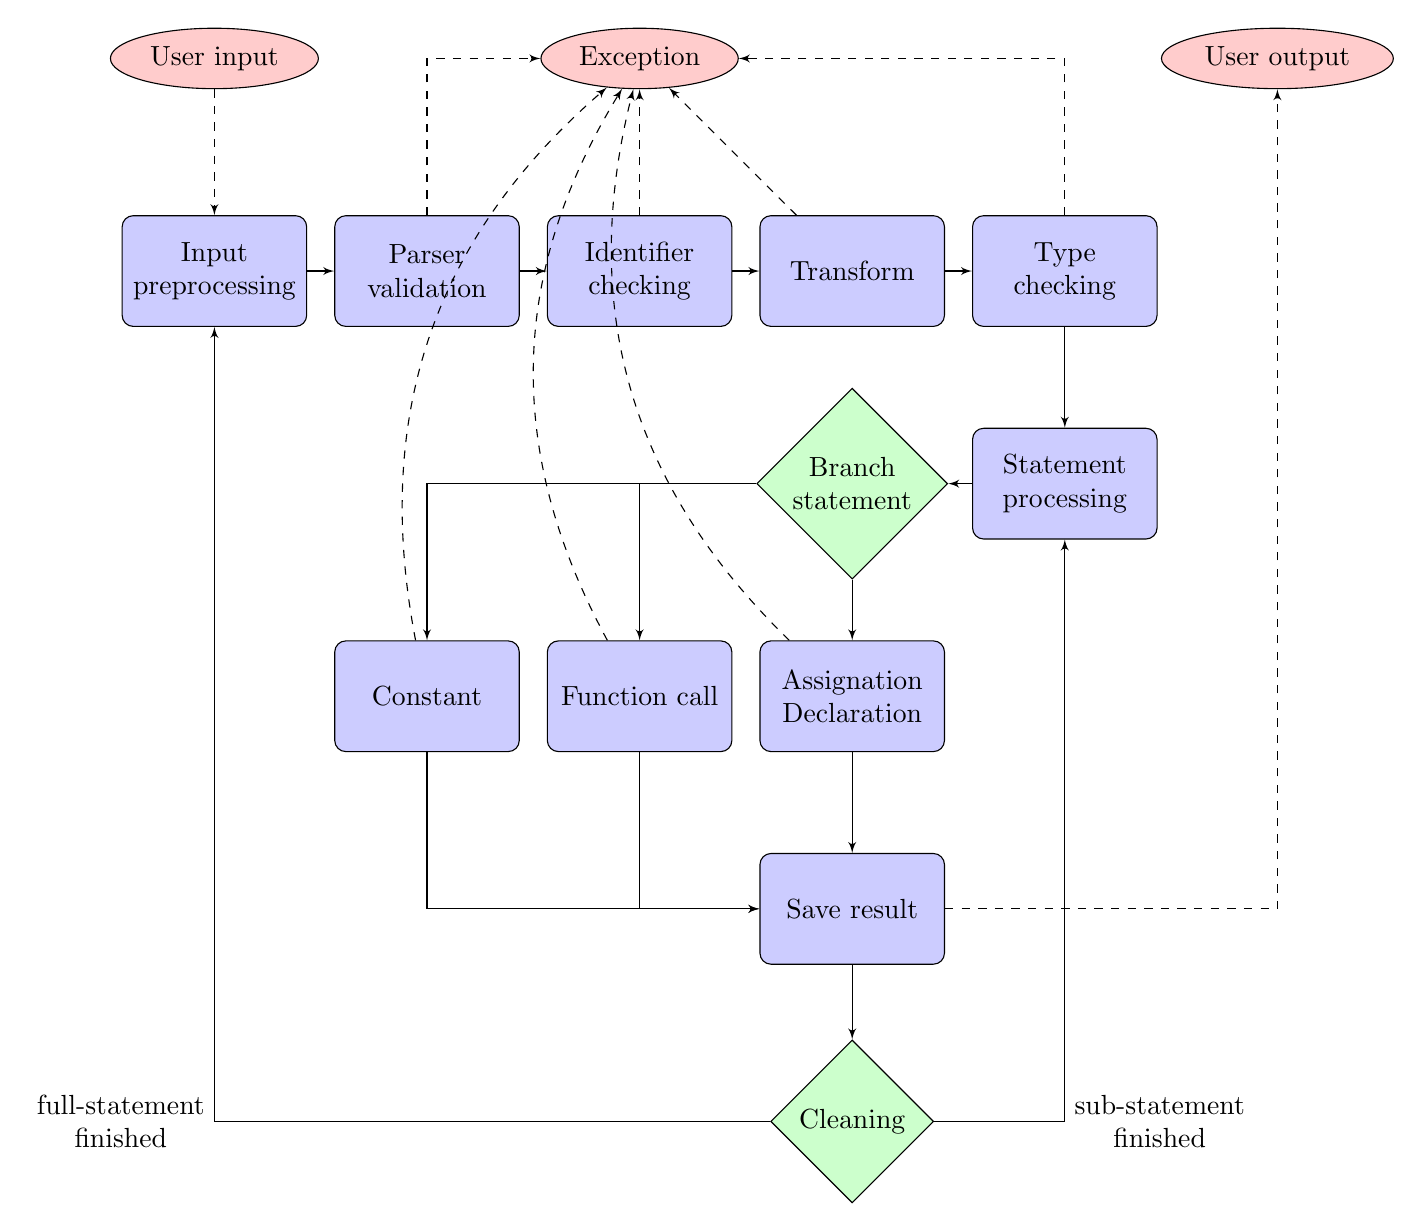
\begin{tikzpicture}[decision/.style = {diamond, draw, fill=green!20, text width=5em, text badly centered, inner sep=0pt}, block/.style = {rectangle, draw, fill=blue!20, text width=6em, text centered, rounded corners, minimum height=4em}, line/.style = {draw, -latex'}, cloud/.style = {draw, ellipse,fill=red!20, minimum height=2em}, node distance = 2.7cm,auto]
					\node[cloud] (input) {User input};
					\node[block,below of=input] (preprocessor) {Input preprocessing};
					\node[block,right of=preprocessor] (parser) {Parser validation};
					\node[block,right of=parser] (identifier) {Identifier checking};
					\node[cloud,above of=identifier] (exception) {Exception};
					\node[block,right of=identifier] (transformation) {Transform};
					\node[block,right of=transformation] (type) {Type checking};
					\node[block,below of=type] (parameter) {Statement processing};
					\node[decision,left of=parameter] (execute) {Branch statement};
					\node[block,below of=execute] (assign) {Assignation Declaration};
					\node[block,left of=assign] (function) {Function call};
					\node[block,left of=function] (constant) {Constant};
					\node[block,below of=assign] (result) {Save result};
					\node[decision,below of=result] (clean) {Cleaning};
					\node[cloud,right of=type,above of=type] (output) {User output};
					
					\path[line,dashed] (input) -- (preprocessor);
					\path[line,dashed] (parser) |- (exception);
					\path[line,dashed] (identifier) -- (exception);
					\path[line,dashed] (type) |- (exception);
					\path[line,dashed] (transformation) -- (exception);
					\path[line,dashed] (function) edge[bend left] (exception);
					\path[line,dashed] (constant) edge[bend left] (exception);
					\path[line,dashed] (assign) edge[bend left] (exception);
					\path[line] (preprocessor) -- (parser);
					\path[line] (parser) -- (identifier);
					\path[line] (identifier) -- (transformation);
					\path[line] (transformation) -- (type);
					\path[line] (type) -- (parameter);
					\path[line] (parameter) -- (execute);
					\path[line] (execute) -| (function);
					\path[line] (execute) -- (assign);
					\path[line] (execute) -| (constant);
					\path[line] (function) |- (result);
					\path[line] (assign) -- (result);
					\path[line] (constant) |- (result);
					\path[line] (result) -- (clean);
					\path[line] (clean) -| node[align=center,right] {sub-statement\\finished} (parameter);
					\path[line] (clean) -| node[align=center] {full-statement\\finished} (preprocessor);
					\path[line,dashed] (result) -| (output);
				\end{tikzpicture}
				\caption{Flux des données dans l'interpréteur}
			\end{figure}
			
			Détaillons chacune de ces étapes:
			\begin{enumerate}
				\item \textbf{Input preprocessing} - On récupère les entrées utilisateur dans un tampon.
				\begin{enumerate}
					\item \textbf{Trim} - On enlève tous les espaces inutiles, c'est-à-dire tous les espaces sauf ceux dans les constantes littérales de type \textit{String}, et celui qui sépare le type de l'identifiant dans les déclarations.
					\item \textbf{Statement per statement} - On envoie au parseur une commande à la fois (les traitements sont séparés par des ';').
				\end{enumerate}
				\item \textbf{Parser validation} - On vérifie la syntaxe de la commande et on extrait des informations utiles pour la suite (tokens), voir section~\ref{subsec:implementation-du-parseur}.
				\item \textbf{Identifier checking} - On connaît les différents identifiants présents dans la commande (noms de variable, noms de fonction), on peut tout de suite vérifier leur existence.
				\item \textbf{Transform} - On transforme la commande en arbre d'appels, plus de détails dans la section~\ref{subsec:regles-de-transformation}.
				\item \textbf{Type checking} - On vérifie la concordance des types (statique), plus de détails dans la section~\ref{subsubsec:verification-des-types}.
				\item \textbf{Statement processing} - La commande a été décomposée en plusieurs sous-traitements (arbre d'appels, \ref{subsubsec:arbre-d-appels-des-traitements}), on effectue d'abord les feuilles avant de remonter.
				\begin{enumerate}
					\item \textbf{Branch statement} - On sélectionne le bon traitement en fonction de son type.
					\begin{itemize}
						\item \textbf{Constant} - On créé une variable temporaire avec la valeur de la constante, voir section~\ref{subsubsec:table-des-temporaires}.
						\item \textbf{Function call} - On appelle la fonction et on sauve son résultat dans une variable temporaire.
						\item \textbf{Assignation} - On assigne une valeur à une variable, voir section~\ref{subsubsec:table-des-variables}.
						\item \textbf{Declaration} - Pareil que l'assignation, mais avec création de l'identifiant au préalable.
					\end{itemize}
					\item \textbf{Save result} - On transforme l'arbre d'appels avec les nouvelles valeurs/variables. Si c'est la fin de la commande, on indique à l'utilisateur que le résultat de la commande est prêt
					\item \textbf{Cleaning} - On supprime les variables temporaires qui ne sont plus utiles. Si c'était un sous-traitement, on passe au prochain sous-traitement (6), sinon on passe à la prochaine commande (1)
				\end{enumerate}
			\end{enumerate}
			
		\subsection{Implémentation du parseur}
			\label{subsec:implementation-du-parseur}
			\textcolor{red}{Boost.Spirit toussa todo blabla ...}
		
		\subsection{Mémoire virtuelle} 
			\label{subsec:memoire-virtuelle}
			Dans le flux de données, certaines étapes nécessitent l'utilisation d'une mémoire afin de gérer les variables (temporaires ou non). Dans cette section nous allons préciser comment cela va être géré.\\
			
			Chaque type du langage possède son pendant en C++, voici un tableau résumant cela:\\
			
			\begin{figure}[H]
				\centering
				\begin{tabular}{r|l}
					Type & Equivalent C++\\ \hline\hline
					\texttt{Boolean} & \texttt{bool}\\
					\texttt{Integer} & \texttt{int}\\
					\texttt{Float} & \texttt{float}\\
					\texttt{String} & \texttt{std::string}\\
					\texttt{Number} & voir section~\ref{subsubsec:number-edge-et-vertex}\\
					\texttt{Array} & voir section~\ref{subsubsec:tableau-dynamique-heterogene}\\
					\texttt{Graph} & voir section~\textcolor{red}{ajouter ref}\\
					\texttt{Vertex} & voir section~\ref{subsubsec:number-edge-et-vertex}\\
					\texttt{Edge} & voir section~\ref{subsubsec:number-edge-et-vertex}
				\end{tabular}
			\end{figure}
			
			\subsubsection{Table des variables}
				\label{subsubsec:table-des-variables}
				Notre interpréteur a besoin de créer des variables afin de pouvoir les manipuler au fur et à mesure des traitement. Une variable est définie par trois informations:
				
				\begin{enumerate}
					\item un type
					\item un identifiant
					\item une valeur
				\end{enumerate}
				
				Pour stocker ces informations, on va utiliser une table de variables qui nous permettra de répondre à différentes questions:
				
				\begin{itemize}
					\item Quelles sont les variables déjà créées?
					\item Quel est le type d'une variable?
					\item Une variable existe-t-elle?
					\item Quelle est la valeur d'une variable?
				\end{itemize}
				
				Le C++ étant un langage fortement typé, on est obligé d'utiliser une approche à base de \texttt{if-else/switch}. Voici un exemple d'implémentation (qui pourrait être \textit{templatisé}):
				
				\begin{lstlisting}
					struct Table {
						enum class Type { Integer, String /* , ... */ };
						map<string, Type> names;
						map<string, int> ints;
						map<string, string> strings;
						// ...
						
						void set(string const &name, int value) {
							if(exists(name) && typeOf(name) != Type::Integer)
								/* bad type exception */;
							names[name] = Type::Integer;
							ints[name] = value;
						}
						
						void set(string const &name, string const &value) {
							// ...
						}
						// ...
						
						bool exists(string const &name) const {
							return names.find(name) != names.end();
						}
						
						Type typeOf(string const &name) const {
							if(!exists(name))
								/* not found exception */;
							return names.find(name)->second;
						}
						
						void erase(string const &name) {
							switch(typeOf(name)) {
								case Type::Integer: ints.erase(name); break;
								case Type::String: strings.erase(name); break;
							}
						}
						
						int getInteger(string const &name) const {
							if(typeOf(name) != Type::Integer)
								/* cast exception */;
							return ints.find(name)->second;
						}
						// ...
					};
				\end{lstlisting}
				
				Cette solution répond à toutes nos questions et a l'avantage d'être assez simple (et typée), une autre approche à base de \texttt{void*} est possible et est présentée dans la section~\ref{subsubsec:tableau-dynamique-heterogene} sur les tableaux dynamiques hétérogènes. Notons qu'il peut être pertinent d'utiliser une autre structure que \texttt{map} pour le stockage des identifiants, par exemple un ternary search tries qui faciliterait l'auto-complétion pour les variables.
			
			\subsubsection{Table des temporaires}
				\label{subsubsec:table-des-temporaires}
				Certains traitements seront composés de plusieurs sous-traitements, les résultats de ceux-ci seront stockés dans des variables qui doivent avoir une durée de vie limitée à la durée du traitement. Une approche simple et efficace est d'utiliser une \texttt{std::stack<Table>} (voir section~\ref{subsubsec:table-des-variables}) sur laquelle on \textit{push} à l'entrée du traitement et on \textit{pop} à sa sortie.\\
				
				Ici nous développons juste l'idée générale, mais concrètement les variables temporaires et non temporaires doivent être accessible de la même manière indépendamment de leur genre. Par conséquent une tables des variables générale englobera les deux genres, et fournira une interface commune permettant de manipuler les deux.
				
			\subsubsection{Tableau dynamique hétérogène}
				\label{subsubsec:tableau-dynamique-heterogene}
				Le tableau dynamique hétérogène (TDH dans la suite de cette section) pose un problème majeur: le C++ est un langage fortement typé. Cependant plusieurs solutions s'offrent à nous pour créer un TDH:
				
				\begin{enumerate}
					\item Un \texttt{std::vector<boost::any>} (\texttt{std::any} étant prévu pour C++17)
					\item Un \texttt{std::vector<std::pair<std::type\_index, void*> >}
					\item Un \texttt{std::vector<std::pair<TypeEnum, void*> >}
				\end{enumerate}
				
				La solution (1) est sans doute la plus propre ainsi que la plus facile, cependant elle ajoute une dépendance avec Boost et elle partage plusieurs problèmes avec la solution (2) que l'on va voir tout de suite.\\
				
				La solution (2) utilise un mécanisme de C++ (l'opérateur \texttt{typeid}) afin de savoir quel est le type réel caché derrière le \texttt{void*}, cela permet un code assez générique. Cependant pour chaque valeur, on doit attacher un objet \texttt{std::type\_index} (lui-même composé d'un \texttt{std::type\_info}), et faire des appels à \texttt{typeid}, cela ajoute un surcoût en temps et en mémoire par rapport à la solution (3).\\
				
				La solution (3) est donc celle retenue pour implémenter un TDH. On créé simplement une énumération contenant les types acceptés dans le TDH, et chaque \texttt{void*} est associé à une valeur de cette énumération. Voici un exemple d'implémentation:
				
				\begin{lstlisting}
					class Array {
					public:
						enum class Type { Boolean, Integer, String /*, ...*/ };
						typedef std::pair<Type, void*> value_type;
						
						// constructeur de copie, etc.
						// ...
						
						~Array() {
							for(value_type& value : values) {
								switch(value.first) {
									case Type::Boolean:
										delete (bool*)value.second;
										break;
									case Type::Integer:
										delete (int*)value.second;
										break;
									case Type::String:
										delete (std::string*)value.second;
										break;
									// ...
								}
							}
						}
						
						size_t size() const {
							return values.size();
						}
						
						void add(int *value) { 
							// value doit provenir d'un 'new'
							values.push_back(std::make_pair(Type::Integer, (void*)value));
						}
						
						void add(int value) {
							add(new int(value));
						}
						// ...
						
						Type typeOf(size_t i) const {
							return values.at(i).first;
						}
						
						int getInteger(size_t i) const {
							if(typeOf(i) != Type::Integer)
								throw /* cast exception */;
							return *(int*)values.at(i).second;
						}
						// ...
						
					private:
					
						std::vector<value_type> values;
					};
				\end{lstlisting}
				
				Cette solution est assez verbeuse, cependant la complexité en temps et en mémoire est très bonne. En ce qui concerne les \texttt{delete}, il est obligatoire de faire le cast avant, sinon le destructeur de l'objet détruit n'est pas appelé.\\
				
				Évidemment l'utilisateur du TDH est obligé de faire des \texttt{switch/if-else} dans son code, cependant ce problème vaut pour chacune des trois solutions et est inhérent au C++.  
				
			\subsubsection{Number, Edge et Vertex}
				\label{subsubsec:number-edge-et-vertex}
				\textbf{Number} - Selon la grammaire, certains nombres peuvent soit être un entier, soit un flottant. Il peut également être intéressant pour certains algorithmes de savoir si ces nombres sont entiers ou non (pour les flots notamment). Pour ces deux raisons, il est nécessaire d'avoir un type \texttt{Number} pouvant stocker les deux types de représentations. Voici deux propositions (incomplètes):
				
				\begin{lstlisting}
					// solution 1
					struct Number {
						enum : char { Integer, Float } tag;
						union { int int_; float float_; };
						Number() : Number(0) {}
						Number(int i) : tag(Integer), int_(i) {}
						Number(float f) : tag(Float), float_(f) {}
						Number(double f) : tag(Float), float_(f) {}
						// ...
					};
					
					// solution 2
					struct Number2 {
						typedef float T;
						T value;
						Number2(T v = T(0)) : value(v) {}
						operator T() const { return value; }
						operator T&() { return value; }
						explicit operator int() const { return value; }
						bool isInt() const { return modf(value, nullptr) == 0.f; } // +/- epsilon
						bool isFloat() const { return !isInt(); }
						// ...
					};
				\end{lstlisting}
				
				La solution (1) a l'avantage d'être plus sûre au niveau du typage, cependant à l'utilisation elle demande davantage de conditions. La solution (2) est plus naturelle à l'utilisation et utilise deux fois moins de place en mémoire que la solution (1), mais le test \texttt{isInt()} prend plus de temps. A partir de là, on a choisi la solution (2) pour ses avantages et car les accès à \texttt{value} seront plus courants que les tests \texttt{isInt()}.\\
								
				\textbf{Vertex} - Le type \texttt{Vertex} pose un problème majeur: certains de ses attributs sont optionnels. Voici donc une solution naturelle:
				
				\begin{lstlisting}
					struct Vertex {
						int id;
						std::string label;
						Number weight;
						Number minCapacity;
						Number maxCapacity;
						bool active[4]; // ~ un bool par attribut optionnel
						// ...
					};
				\end{lstlisting}
				
				Le souci avec cette approche est que les attributs optionnels sont construits même s'ils ne sont pas utilisés, par ailleurs sur mon ordinateur \texttt{sizeof(Vertex) == 36}. Cela implique une utilisation inutile en ressources pour des attributs qui ne seront pas forcément utilisés.\\
				
				Afin d'éviter ces problèmes, on peut approcher le problème avec des pointeurs (égaux à \texttt{nullptr} s'ils ne sont pas utilisés):
				
				\begin{lstlisting}
					struct Vertex {
						int id;
						std::string* label;
						Number* weight;
						Number* minCapacity;
						Number* maxCapacity;
						// ...
					};
				\end{lstlisting}
				
				A présent, \texttt{sizeof(Vertex) == 20} (sur ma machine) et les objets ne sont plus construits inutilement. Le gain en ressource n'est pas négligeable, cependant cette structure n'est pas très agréable à utiliser telle quelle (gestion de l'allocation/désallocation, déréférencement). Pour palier à cela, on délègue la gestion du pointeur à une autre classe, dont voici un aperçu:
				
				\begin{lstlisting}
					template<typename T>
					struct Optional {
						T* value;
						
						// constructeur/destructeur
						Optional() : value(nullptr) {}
						~Optional() { delete value; }
						
						// operations de copie
						Optional(const Optional &o) : value(nullptr) { 
							if(o.value) value = new T(*o.value); 
						}
						Optional(Optional &&o) : value(move(o.value)) {}
						Optional &operator=(const Optional &o) {
							if(this != &o) {
								delete value;
								value = nullptr;
								if(o.value) value = new T(*o.value);
							}
							return *this;
						}
						Optional &operator=(Optional &&o) {
							if(this != &o) {
								delete value;
								value = move(o.value);
							}
							return *this;
						}
						
						// affectations et constructions
						Optional(const T& v) { value = new T(v); }
						Optional(T&& v) : value(new T(move(v))) {}
						Optional &operator=(const T &v) {
							if(value) *value = v;
							else value = new T(v);
							return *this;
						}
						Optional &operator=(T &&v) {
							if(value) *value = move(v);
							else value = new T(move(v));
							return *this;
						}
						
						// ...
						// operateurs d'acces, etc.
						// ...
					};
					
					struct Vertex {
						int id;
						Optional<string> label;
						Optional<Number> weight;
						Optional<Number> minCapacity;
						Optional<Number> maxCapacity;
						// ...
					};
				\end{lstlisting} 
				
				Notre type \texttt{Vertex} est à présent élégant, et plus efficace en terme de ressources. Notons que \texttt{std::optional<>} sera disponible en C++17.\\
				
				\textbf{Edge} - En ce qui concerne le type \texttt{Edge}, on peut utiliser la même démarche que pour le type \texttt{Vertex}:
				
				\begin{lstlisting}
					struct Edge {
						enum Connection : char { Unidirectional, Bidirectional };
						int a, b;
						Connection conn;
						Optional<Number> weight;
						Optional<string> label;
						Optional<Number> minCapacity;
						Optional<Number> maxCapacity;
						// ...
					};
				\end{lstlisting}
				
				Nos types "simples" sont maintenant définis, notons que les exemples d'implémentation ci-dessus ne sont pas complets, mais ils montrent l'approche générale.
				
		\subsection{Table des fonctions}
			\label{subsec:table-des-fonctions}
			Dans le flux de données, l'étape \textit{Function call} nécessite d'appeler, d'exécuter et de récupérer le résultat d'une fonction. Dans cette section nous allons préciser comment cela va être fait.\\
			
			Voici l'idée avec un bout de code qui devrait pouvoir être exécuté:
			
			\begin{lstlisting}
					// algorithme independant de l'interpreteur
					Graph dijkstra(const Graph &graph, const Vertex &origin) {
						// ...
					}
			
					// interfacage dans la table des fonctions
					functions.add("dijkstra", &dijkstra);
					
					// appel a la fonction depuis l'interpreteur
					functions.call("dijkstra", "pcc", {"g", "v1"});
			\end{lstlisting}
			
			Ce \texttt{call} va chercher les variables \textit{g} et \textit{v1} dans la table des variables, puis appelle la fonction \texttt{dijkstra} avant de sauver le résultat dans la table des variables sous le nom \textit{pcc}.\\
			
			La difficulté, comme d'habitude, est de lié le côté dynamique de l'interpréteur avec le côté fortement typé de C++. Le deuxième problème est d'avoir un interfaçage facile à faire côté utilisateur, afin que l'ajout de nouvelle fonction soit rapide et élégant.\\
			
			Une liste des fonctions interfacées dans l'application se trouve dans l'annexe~\ref{subsec:annexes-fonctions-incluses}. 
			
			\subsubsection{Interfaçage}
				\label{subsubsec:interfacage}
				Afin de répondre aux demandes de la table des fonctions (voir section~\ref{subsec:table-des-fonctions}), on va utilise deux outils que le C++ nous offre: l'héritage (avec polymorphisme) et la spécialisation des \texttt{template}.\\
				
				Un exemple d'implémentation vaut plus qu'un long discours:
				
				\begin{lstlisting}
					// Types geres
					enum class Type { Integer, String /* , ... */ };
					
					// Table des variables (simplifiee)
					struct VarTable {
						map<string, Type> names;
						map<string, int> ints;
						map<string, string> strings;
						
						void set(string const &name, int value) {
							names[name] = Type::Integer;
							ints[name] = value;
						}
						
						void set(string const &name, string const &value) {
							names[name] = Type::String;
							strings[name] = value;
						}
					};
					
					// Acces aux variables specialise
					template<typename> struct Fetcher;
					
					template<> struct Fetcher<int> {
						static int get(string const &name, VarTable &var) {
							return var.ints[name];
						}
					};
					
					template<> struct Fetcher<string> {
						static string const &get(string const &name, VarTable &var) {
							return var.strings[name];
						}
					};
					
					// Enleve les 'const' et les '&' sur un type
					template<typename T> struct RemoveAll {
						typedef typename remove_const<typename remove_reference<T>::type>::type type;
					};
					
					// Classe abstraite pour l'appel a une fonction
					struct FuncBase {
						virtual ~FuncBase() {}
						virtual void execute(string const&, vector<string> const&, VarTable&) = 0;
					};
					
					// Type inutile pour les specialisations de la classe Func
					struct Empty {};
					
					// Classe appelant notre fonction
					// (ici avec 2 parametres max, mais peut etre etendu)
					template<typename R, typename P1 = Empty, typename P2 = Empty>
					struct Func : FuncBase {
						function<R(P1, P2)> f;
						Func(R(*f)(P1, P2)) : f(f) {}
						virtual ~Func() {}
						
						// on appelle la fonction avec ses parametres
						void execute(string const &dst, vector<string> const &params, VarTable &var) {
							P1 p1 = Fetcher<typename RemoveAll<P1>::type>::get(params[0], var);
							P2 p2 = Fetcher<typename RemoveAll<P2>::type>::get(params[1], var);
							var.set(dst, f(p1, p2));
						}
					};
					
					// Meme chose mais pour 1 parametre
					template<typename R, typename P1>
					struct Func<R, P1, Empty> : FuncBase {
						function<R(P1)> f;
						Func(R(*f)(P1)) : f(f) {}
						virtual ~Func() {}
						void execute(string const &dst, vector<string> const &params, VarTable &var) {
							P1 p1 = Fetcher<typename RemoveAll<P1>::type>::get(params[0], var);
							var.set(dst, f(p1));
						}
					};
					
					// Meme chose pour 0 parametre
					template<typename R>
					struct Func<R, Empty, Empty> : FuncBase {
						function<R()> f;
						Func(R(*f)()) : f(f) {}
						virtual ~Func() {}
						void execute(string const &dst, vector<string> const &params, VarTable &var) {
							var.set(dst, f());
						}
					};
					
					// On rend la creation de Func simple pour l'utilisateur
					template<typename R, typename P1, typename P2>
					FuncBase *makeFunc(R(*f)(P1, P2)) {
						return new Func<R, P1, P2>(f);
					}
					template<typename R, typename P1>
					FuncBase *makeFunc(R(*f)(P1)) {
						return new Func<R, P1>(f);
					}
					template<typename R>
					FuncBase *makeFunc(R(*f)()) {
						return new Func<R>(f);
					}
					
					// Table des fonctions (simplifiee)
					struct FuncTable {
						VarTable &var;
						map<string, FuncBase*> names;
						
						FuncTable(VarTable &var) : var(var) {}
						~FuncTable() { 
							for(auto p : names) 
								delete p.second; 
						}
						
						// on appelle la fonction 'name'
						void execute(string const &name, string const &dst, vector<string> const &params) {
							// verifications eventuelles
							// ...
							
							names[name]->execute(dst, p, var);
						}
					};
					
					// Fonctions de test
					int add(int a, int b) { return a + b; }
					int inv(int a) { return -a; }
					int len(string const &s) { return s.size(); }
					string hw() { return "helloworld"; }
					
					int main()
					{
						// On cree des variables
						VarTable var;
						var.names["a"] = Type::Integer;
						var.ints["a"] = 2;
						var.names["b"] = Type::Integer;
						var.ints["b"] = 3;
						
						// On interface les fonctions
						FuncTable func(var);
						func.names["add"] = makeFunc(&add);
						func.names["inv"] = makeFunc(&inv);
						func.names["len"] = makeFunc(&len);
						func.names["hw"] = makeFunc(&hw);
						
						// Affichera: -5
						func.execute("add", "c", {"a", "b"});
						func.execute("inv", "c", {"c"});
						cout << var.ints["c"] << endl;
						
						// Affichera: helloworld/10
						func.execute("hw", "s", {});
						func.execute("len", "l", {"s"});
						cout << var.strings["s"] << "/" << var.ints["l"] << endl;
						
						return 0;
					}
				\end{lstlisting}
				
				Le coeur de la solution est la classe de base abstraite \texttt{FuncBase} dont hérite la classe \textit{templatisée} \texttt{Func} qui effectue l'appel effectif à la fonction interfacée. On remarque que cela fonctionne bien, et que côté utilisateur l'ajout d'une nouvelle fonction est très agréable . Il est de plus encore possible d'ajouter des informations (nom, arité, types, ...) sur chacune des fonctions interfacée.\\
				
				Remarque: L'implémentation ci-dessus utilise la spécialisation des \textit{template} et est limitée en terme de nombre de paramètres que les fonctions interfacées peuvent avoir (même si c'est facilement extensible). Une autre approche, plus générique encore, est d'utiliser les \textit{variadic template} de C++11, cependant cette solution est plus compliquée à développer, le choix est donc laissé au développeur.
				
			\subsubsection{Surcharge}
				Nous avons vu comment interfacer des fonctions simplement, cependant il n'est pour l'instant pas possible d'interfacer plusieurs fonctions ayant le même nom mais une signature différente. Nous allons voir à présent comment cela va être géré.\\
				
				Il existe sans doute plusieurs manières de faire cela, une solution simple consiste à: 
				
				\begin{itemize}
					\item modifier la \texttt{map} dans \texttt{FuncTable} en une \texttt{multimap}
					\item ajouter une méthode abstraite \texttt{bool match(vector<string> const \&params, VarTable \&var)} dans \texttt{FuncBase}
					\item modifier la méthode \texttt{execute} de \texttt{FuncTable} afin qu'elle exécute la première \texttt{FuncBase} qui \texttt{match} les paramètres passés
				\end{itemize}
				
				Un test de faisabilité a été fait et cela marche très bien, on ne mets pas le code entier ici car c'est le même que précédemment. Cependant la méthode \texttt{match} est quand même intéressante:
				
				\begin{lstlisting}
					// ...
					
					template<typename T> struct TypeOf;
					template<typename T> struct TypeOf<T&> : TypeOf<T> {};
					template<typename T> struct TypeOf<const T> : TypeOf<T> {};
					template<> struct TypeOf<int> { static constexpr Type value = Type::Integer; };
					template<> struct TypeOf<string> { static constexpr Type value = Type::String; };
					
					// ...
					
						// dans la classe Func a deux parametres (heritant de FuncBase)
						virtual bool match(vector<string> const& params, VarTable& var) {
							return params.size() == 2
								&& TypeOf<P1>::value == var.names[params[0]]
								&& TypeOf<P2>::value == var.names[params[1]];
						}
					
					// ...
				\end{lstlisting}
				
				Une autre solution serait d'utiliser une \texttt{map<pair<string, vector<Type> >, FuncBase*>} et de construire la signature (\texttt{vector<Type>}) lors de l'interfaçage et lors de l'appel à une fonction.
				
		\subsection{Règles de transformation}
			\label{subsec:regles-de-transformation}
			Dans cette section nous allons préciser les règles de transformation de l'étape \textit{Transform} du flux de données, ainsi que ce que cela va apporter. Pour commencer, voici quelques exemples de transformations possibles:
			
			\begin{figure}[H]
				\centering
				\begin{tabular}{rcl}
					\texttt{(1::3)} & $\rightarrow$ & \texttt{\_vertex\_create(1,-,3)}\\
					\texttt{(0->1:2::3)} & $\rightarrow$ & \texttt{\_edge\_create\_unidirectional(0,1,2,-,3)}\\
					\texttt{[1,2,3]} & $\rightarrow$ & \texttt{\_array\_add(\_array\_add(\_array\_add(\_array\_create(),1),2),3)}\\
					\texttt{\{\#3,0->1,1->2:6\}} & $\rightarrow$ & \texttt{\{1,2,3,0->1,1->2:6\}}\\
												 & $\rightarrow$ & \texttt{\{[(1),(2),(3),(0->1),(1->2:6)]\}}\\
												 & $\rightarrow$ & \texttt{\_graph\_create(\_array\_add(...))}\\
					\texttt{g+=(3)} & $\rightarrow$ & \texttt{g=\_graph\_add(g,\_vertex\_create(3,-,-,-,-))}\\
				\end{tabular}
			\end{figure}
			
			Comme on le voit, le but est de passer de la syntaxe du langage à une représentation sous forme de fonctions. Plus précisément sous une forme d'arbre représentant la hiérarchie d'appel des différents traitements et sous-traitements.\\
			
			On va prendre un exemple de départ complet, et on va développer l'arbre correspondant. Voici notre exemple qui contient tout ce qui nous intéresse:\\
			
			\centering
			\texttt{pcc=dijkstra(\{v0,1:Yverdon,e01,2,0->2:9,1<-2:3\},v0)} (avec \texttt{v0=(0)} et \texttt{e01=(0->1)})
			\justify
			
			\begin{itemize}
				\item assignation (avec déclaration)
				\item appel de fonction
				\item identifiant passé en paramètre
				\item temporaires passés en paramètre
				\item constantes littérales\\
			\end{itemize}
			
			Et voici l'arbre correspondant:
			
			\begin{figure}[H]
				\centering
				\begin{forest}
				value/.style={rectangle,draw=none,rounded corners=1mm,fill=gray!10,drop shadow,text centered, anchor=north,text=black}, 
				type/.style={circle,draw=none,fill=orange,circular drop shadow,text centered,anchor=north,text=white}
					[{A},type
						[{pcc},value] 
						[{F},type
							[{dijkstra},value]
							[{F},type
								[{\_g\_c},value]
								[{F},type
									[{\_a\_a},value]
									[{F},type
										[{\_a\_a},value]
										[{F},type
											[{\_a\_a},value]
											[{F},type
												[{\_a\_a},value]
												[{F},type
													[{\_a\_a},value]
													[{F},type
														[{\_a\_a},value]
														[{F},type
															[{\_a\_c},value]
														]
														[{V},type
															[{v0},value]
														]
													]
													[{F},type
														[{\_v\_c},value]
														[{C},type
															[{1},value]
														]
														[{C},type
															[{Yverdon},value]
														]
													]
												]
												[{V},type
													[{e01},value]
												]
											]
											[{F},type
												[{\_v\_c},value]
												[{C},type
													[{2},value]
												]
											]
										]
										[{F},type
											[{\_e\_c\_u},value]
											[{C},type
												[{0},value]
											]
											[{C},type
												[{2},value]
											]
											[{C},type
												[{9},value]
											]
										]
									]
									[{F},type
										[{\_e\_c\_u},value]
										[{C},type
											[{2},value]
										]
										[{C},type
											[{1},value]
										]
										[{C},type
											[{3},value]
										]
									]
								]
							]
							[{V},type
								[{v0},value]
							]
						]
					]	
				\end{forest}
				\caption{Exemple d'arbre d'appels de traitements}
			\end{figure}
			
			NB: on a simplifié les noms des fonctions afin que l'image ne soit pas trop large (\texttt{\_g\_c=\_graph\_create}, \texttt{\_a\_a=\_array\_add}, \texttt{\_a\_c=\_array\_create}, \texttt{\_v\_c=\_vertex\_create} et \texttt{\_e\_c\_u=\_edge\_create\_unidirectional}).\\
			
			Dans ce graphe on a deux types de noeuds, les ronds qui représentent des traitements, et les rectangles qui représentent des valeurs. On remarque qu'on a plusieurs types de traitements:
			
			\begin{figure}[H]
				\centering
				\begin{tabular}{cccc}
					Type & Nom complet & Valeur & Nombre de paramètres\\
					\hline
					A & Assignation & Nom de la variable & 1\\
					F & Fonction & Nom de la fonction & *\\
					C & Constante & Valeur littérale & 0\\
					V & Variable & Nom de la variable & 0\\
				\end{tabular}
			\end{figure}
			
			D'un point de vue structure de données cet arbre est très simple, voici un exemple:
			
			\begin{lstlisting}
					struct Statement {
						enum class Type { A, F, C, V };
						Type type;
						string value;
						vector<Statement> parameters;
					};
			\end{lstlisting}
			
			La création de cet arbre se fait grâce aux \textit{tokens} générés dans la partie \textit{Parser validation} (voir section~\ref{subsec:implementation-du-parseur}), \textcolor{red}{bla bla bla à compléter}
			
			\subsubsection{Fonctions internes}
				La transformation nécessite plusieurs fonctions pour que la suite puisse correctement fonctionner. Nous allons lister ici toutes ces fonctions qui seront par la suite interfacées dans la table des fonctions.\\
				
				Note: les paramètres de type \texttt{T} indiquent qu'il existe une surcharge de la fonction pour chacun des types disponible dans le langage.
				
				\begin{figure}[H]
					\centering
					\begin{tabular}{lll}
						Prototype & Description\\
						\hline
						\texttt{} & \\
					\end{tabular}
				\end{figure}
			
			\subsubsection{Arbre d'appels des traitements}
				\label{subsubsec:arbre-d-appels-des-traitements}
				Maintenant que nous avons un arbre d'appels hiérarchique des traitements, reste à savoir comment nous allons l'utiliser (étapes \textit{Statement processing} et \textit{Save result} du flux de données). Le principe est très simple: 
				
				\begin{enumerate}
					\item On prend le traitement racine
					\item On parcours les paramètres:
					\begin{itemize}
						\item Si c'est un V, on passe
						\item Sinon on effectue le sous-traitement (récursion)
					\end{itemize}
					\item On effectue le traitement racine
				\end{enumerate}
				
				Concrètement on voit que tous les traitements ont besoin d'accéder aux valeurs de leur paramètres, cela ne peut se faire que si le paramètre est une variable. Donc si ce n'est pas une variable, on effectue le traitement associé avant de le sauver dans une variable (temporaire). L'arbre va donc raccourcir au fur et à mesure de l'avancement des sous-traitements.\\
				
				Prenons un exemple simple \texttt{a=1+max(-b,2)} (avec \texttt{b=-3}), qui devient donc \texttt{a=add(1,max(neg(b),2))}. L'arbre va évoluer ainsi (avec en orange le paramètre à traiter, en rouge sa variable résultante et en jaune la récursion):
				
				\begin{figure}[H]
					\centering
					\begin{tabular}{c|c|c}
						\begin{forest}
							[{A},fill=yellow
								[{a}]
								[{F},fill=yellow
									[{add}]
									[{C},fill=orange
										[{1}]
									]
									[{F}
										[{max}]
										[{F}
											[{neg}]
											[{V}
												[{b}]
											]
										]
										[{C}
											[{2}]
										]
									]
								]
							]
						\end{forest}
						&
						\begin{forest}
							[{A},fill=yellow
								[{a}]
								[{F},fill=yellow
									[{add}]
									[{V},fill=red
										[{t0}]
									]
									[{F},fill=yellow
										[{max}]
										[{F},fill=orange
											[{neg}]
											[{V}
												[{b}]
											]
										]
										[{C}
											[{2}]
										]
									]
								]
							]
						\end{forest}
						&
						\begin{forest}
							[{A},fill=yellow
								[{a}]
								[{F},fill=yellow
									[{add}]
									[{V}
										[{t0}]
									]
									[{F},fill=yellow
										[{max}]
										[{V},fill=red
											[{t1}]
										]
										[{C},fill=orange
											[{2}]
										]
									]
								]
							]
						\end{forest}
						\\
						\textbf{début} & \textbf{étape 1} & \textbf{étape 2}\\
						\hline
						&&\\ % pour faire joli
						\begin{forest}
							[{A},fill=yellow
								[{a}]
								[{F},fill=yellow
									[{add}]
									[{V}
										[{t0}]
									]
									[{F},fill=orange
										[{max}]
										[{V}
											[{t1}]
										]
										[{V},fill=red
											[{t2}]
										]
									]
								]
							]
						\end{forest}
						&
						\begin{forest}
							[{A},fill=yellow
								[{a}]
								[{F},fill=orange
									[{add}]
									[{V}
										[{t0}]
									]
									[{V},fill=red
										[{t3}]
									]
								]
							]
						\end{forest}
						&
						\begin{forest}
							[,phantom,s sep=1cm
								[{A},fill=orange
									[{a}]
									[{V},fill=red
										[{t4}]
									]
								]
								[{V},fill=red
									[{a}]
								]
							]
						\end{forest}
						\\
						\textbf{étape 3} & \textbf{étape 4} & \textbf{étapes 5 et fin}\\ 
					\end{tabular}
					\caption{Évolution d'un arbre d'appels des traitements}
				\end{figure} 
				
				NB: les variables \texttt{tX} sont des variables temporaires, elles seront supprimées à la fin du (sous-)traitement qui en avait besoin.\\
				
				Premièrement on voit que cette approche récursive nous permet de bien arriver au résultat escompté, et ce, depuis un traitement qui à la base était très complexe avant sa transformation. Deuxièmement il est important de noter que tout traitement finira toujours par retourner une valeur dans une variable (temporaire ou pas).
			
			\subsubsection{Vérification des types}
				\label{subsubsec:verification-des-types}
				L'arbre d'appel des traitements nous permet d'implémenter également la partie \textit{Type checking} du flux de données. Le but de cette partie est de faire une première vérification sur la concordance des types entre les fonctions et leurs paramètres. Ainsi on évite d'effectuer pleins de sous-traitements pour finalement tout annuler car il y a un problème ailleurs dans l'arbre, plus un soucis est détecté tôt, mieux c'est.\\
				
				Cela est possible car les tables des variables et des fonctions nous permet d'obtenir des informations sur leurs contenus. L'algorithme consiste à nouveau en une simple récursion dans l'arbre, et à chaque noeud on vérifie les types.\\
				
				NB: cette vérification ne verra pas tous les problèmes de types, typiquement à cause des tableaux dynamiques hétérogènes.
			
		\subsection{Architecture}
			Un des buts de l'application est de pouvoir travailler sur plusieurs onglets en même temps. Cela implique que chacun aura des variables différentes et indépendantes.\\
			
			L'approche de base est que chaque onglet aura une instance de l'interpréteur:
			
			\begin{figure}[H]
				\centering
				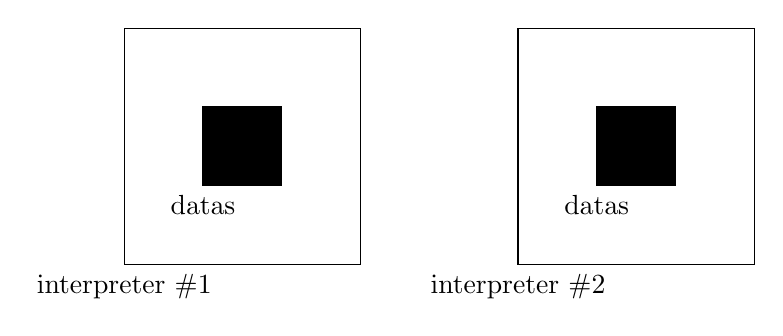
\begin{tikzpicture}
					\draw (0,0) node[anchor=north] {interpreter \#1} rectangle (3,3);
					\draw[fill=black] (1,1) node[anchor=north] {datas} rectangle (2,2);
					
					\draw (5,0) node[anchor=north] {interpreter \#2} rectangle (8,3);
					\draw[fill=black] (6,1) node[anchor=north] {datas} rectangle (7,2);
				\end{tikzpicture}
			\end{figure}
			
			Cette approche a cependant le désavantage de dupliquer l'interpréteur dans la mémoire, alors que celui-ci est le même. Ce qui définit l'état dans lequel l'interpréteur est, c'est les données dans la mémoires virtuelle de celui-ci, c'est-à-dire la table des variables (voir éventuellement la table des fonctions). On peut donc développer une autre solution, très proche des processeurs et de leurs registres:
			
			\begin{figure}[H]
				\centering
				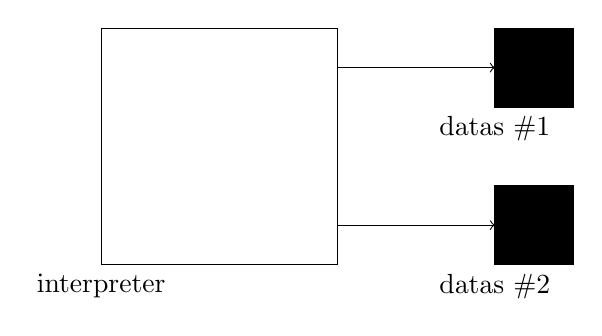
\begin{tikzpicture}
					\draw (0,0) node[anchor=north] {interpreter} rectangle (3,3);
					\draw[fill=black] (5,2) node[anchor=north] {datas \#1} rectangle (6,3);
					\draw[fill=black] (5,0) node[anchor=north] {datas \#2} rectangle (6,1);
					\draw[->] (3,2.5) -- (5,2.5);
					\draw[->] (3,0.5) -- (5,0.5);
				\end{tikzpicture}
				\caption{Architecture générale de l'interpréteur}
			\end{figure}
			
			A présent l'interpréteur n'est plus dupliqué, ainsi chaque onglet aura ses données et il suffira d'indiquer à l'interpréteur quel jeu de données il doit utiliser.
			
			\subsubsection{Interface utilisateur}
				Avant de s'attaquer au diagramme de classes, on peut se poser la question de l'interface qui sera fournie à l'utilisateur de l'interpréteur. Très simplement, celui-ci a besoin de:
				
				\begin{itemize}
					\item Instancier l'interpréteur
					\item Instancier une ou des tables des variables
					\item Connecter l'interpréteur à une table des variables
					\item Interfacer des fonctions avec l'interpréteur (éventuellement)
					\item Envoyer une commande (requête) à interpréter
					\item Récupérer le résultat d'une commande
					\item Connaître les fonctions disponibles
					\item Connaître les variables disponibles
				\end{itemize}
				
				Notons que les résultats peuvent être de plusieurs types: erreur avec message des détails, succès avec le nom de la variable de résultat.
			
			\subsubsection{Diagramme de classes}
			
				\begin{figure}[H]
					\centering
					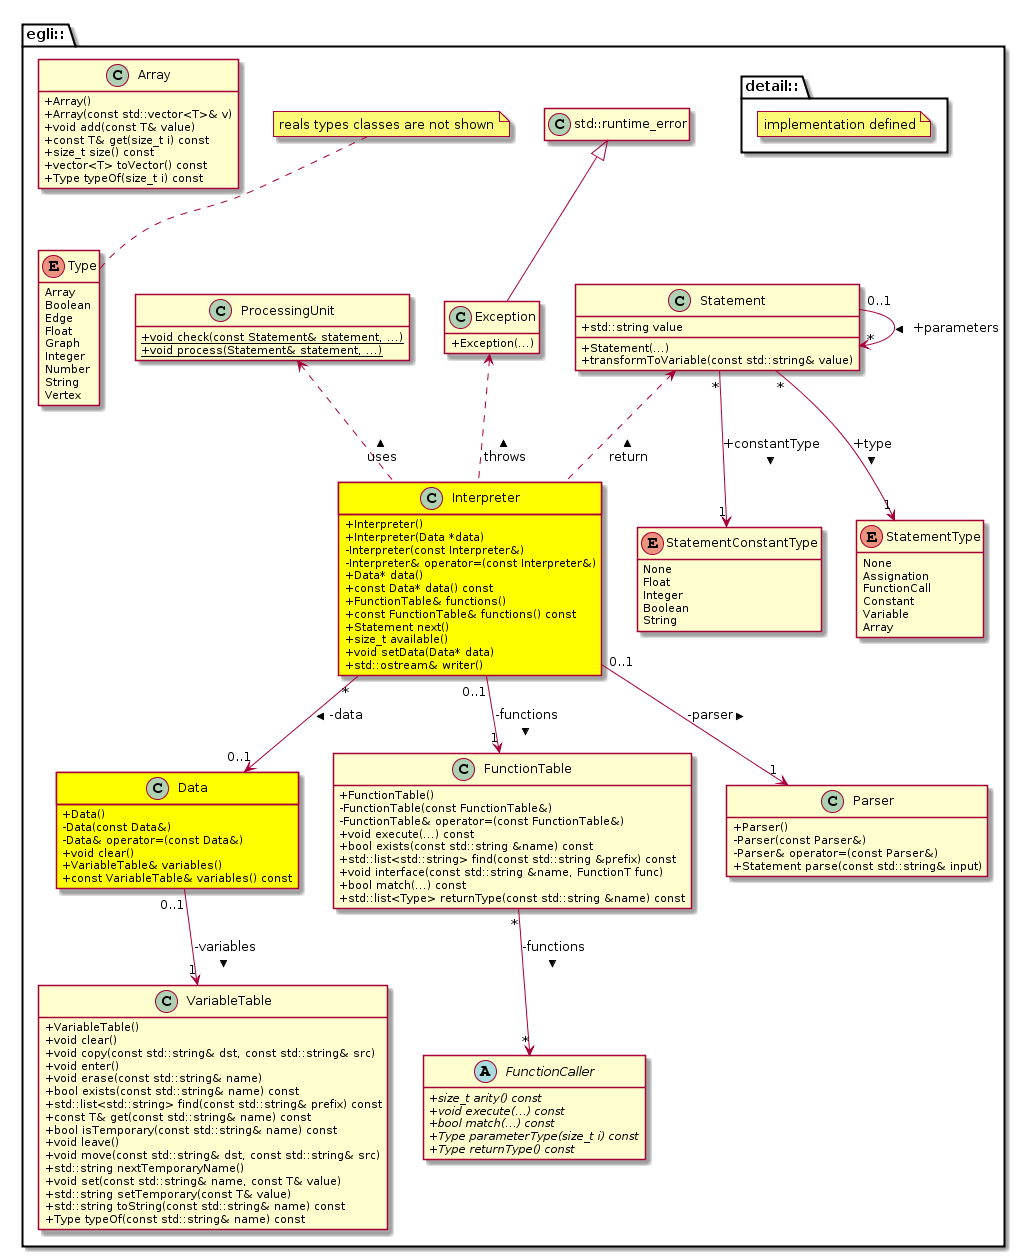
\includegraphics[width=0.9\textheight,angle=90]{Conception/UMLEGLI}
					\caption{Diagramme de classes de l'interpréteur  \cite{plantuml}}
				\end{figure}
				
				Ce diagramme ne montre pas les attributs des classes car l'implémentation de chacune n'est pas fixée comme on a pu le voir dans les sections précédentes. De plus l'interface est là à titre indicative, il est possible qu'il y ait quelques modifications dans les sources. Pour finir certaines classes ont des $\dots$, cela indique que l'on ne sait pas encore à l'heure actuelle ce qu'il y aura à l'intérieur.
			
			\subsubsection{Répertoires}
				L'interpréteur étant une couche indépendante de l'application GUI, nous avons décidé de mettre tout ce qui le concerne dans un \texttt{namespace} du nom de \texttt{egli}, pour \textit{Embeeded GraphY Language Interpreter}.\\
				
				Voici à quoi ressemblera le répertoire de l'interpréteur:
				
				\textcolor{red}{bla bla todo ...}
			
		\subsection{Exemples}
		
	\section{Graphes}
		\subsection{Préface}
		Un graphe est une structure composée d'un ensemble de sommets et d'arêtes/arcs. Il existe différentes familles de graphe, comme les graphes orientés, à flot, biparti, etc., ainsi que différents moyen de les représenter.
		
		Cette section a pour but dans un premier temps de présenter les interfaces à disposition de l'utilisateur pour manipuler des graphes, et dans un second temps, de montrer nos choix de modélisation et d'implémentation de ceux-ci.
		
		\subsection{Sommets et arcs/arêtes}
		
		
		\subsubsection{La classe "Vertex"}
		
		\subsubsection{La classe "Edge"}
		
		\subsection{La classe "Graph"}
		Dans l'optique d'un code modulable, nous avons décidé d'offrir à l'utilisateur différentes interfaces lui permettant la création et la manipulation de graphes. Par exemple, la vue aura besoin de récupérer les sommets et les arêtes d'un graphe pour le dessiner, le parseur voudra probablement créer un graphe après avoir parsé des données, ou encore un algorithme devra parcourir ce graphe pour trouver un plus court chemin.
		
			\subsubsection{Interface utilisateur}
			Voici une ébauche de l'interface permettant la manipulation de graphes :
			\begin{figure}[H]
				\centering
				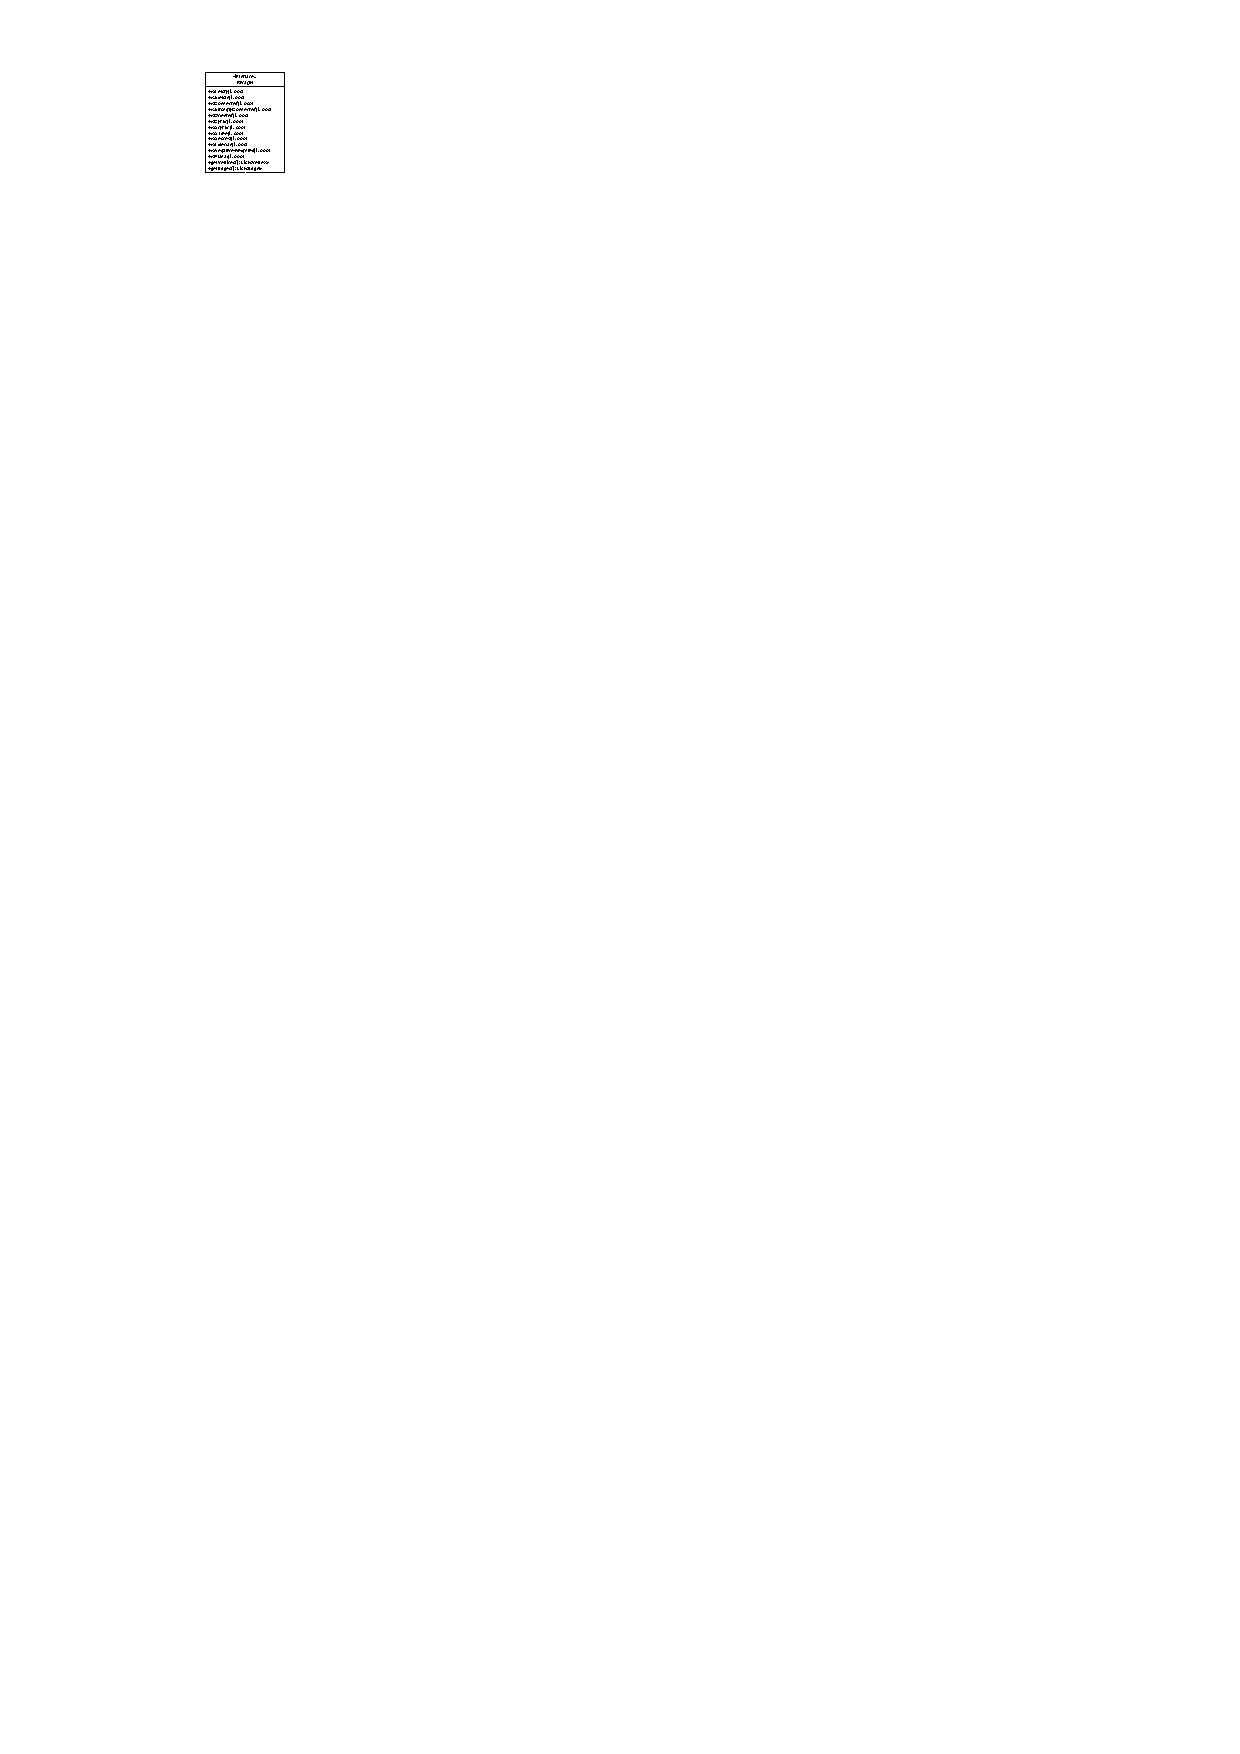
\includegraphics[scale=3.0]{Conception/igraph.pdf}
				\caption{Interface IGraph}
			\end{figure}
			Tout part de cette interface et le but que nous recherchons est qu'elle soit la plus complète possible afin de répondre à tous les besoins de nos utilisateurs. \\
			
			\subsubsection{Types de graphe}
			Concrètement, n'importe quel graphe doit pouvoir implémenter cette interface, d'où la présence d'une classe commune aux graphes. Cette classe nous est utile pour factoriser au maximum les fonctions communes à tout type de graphe.
			\begin{figure}[H]
				\centering
				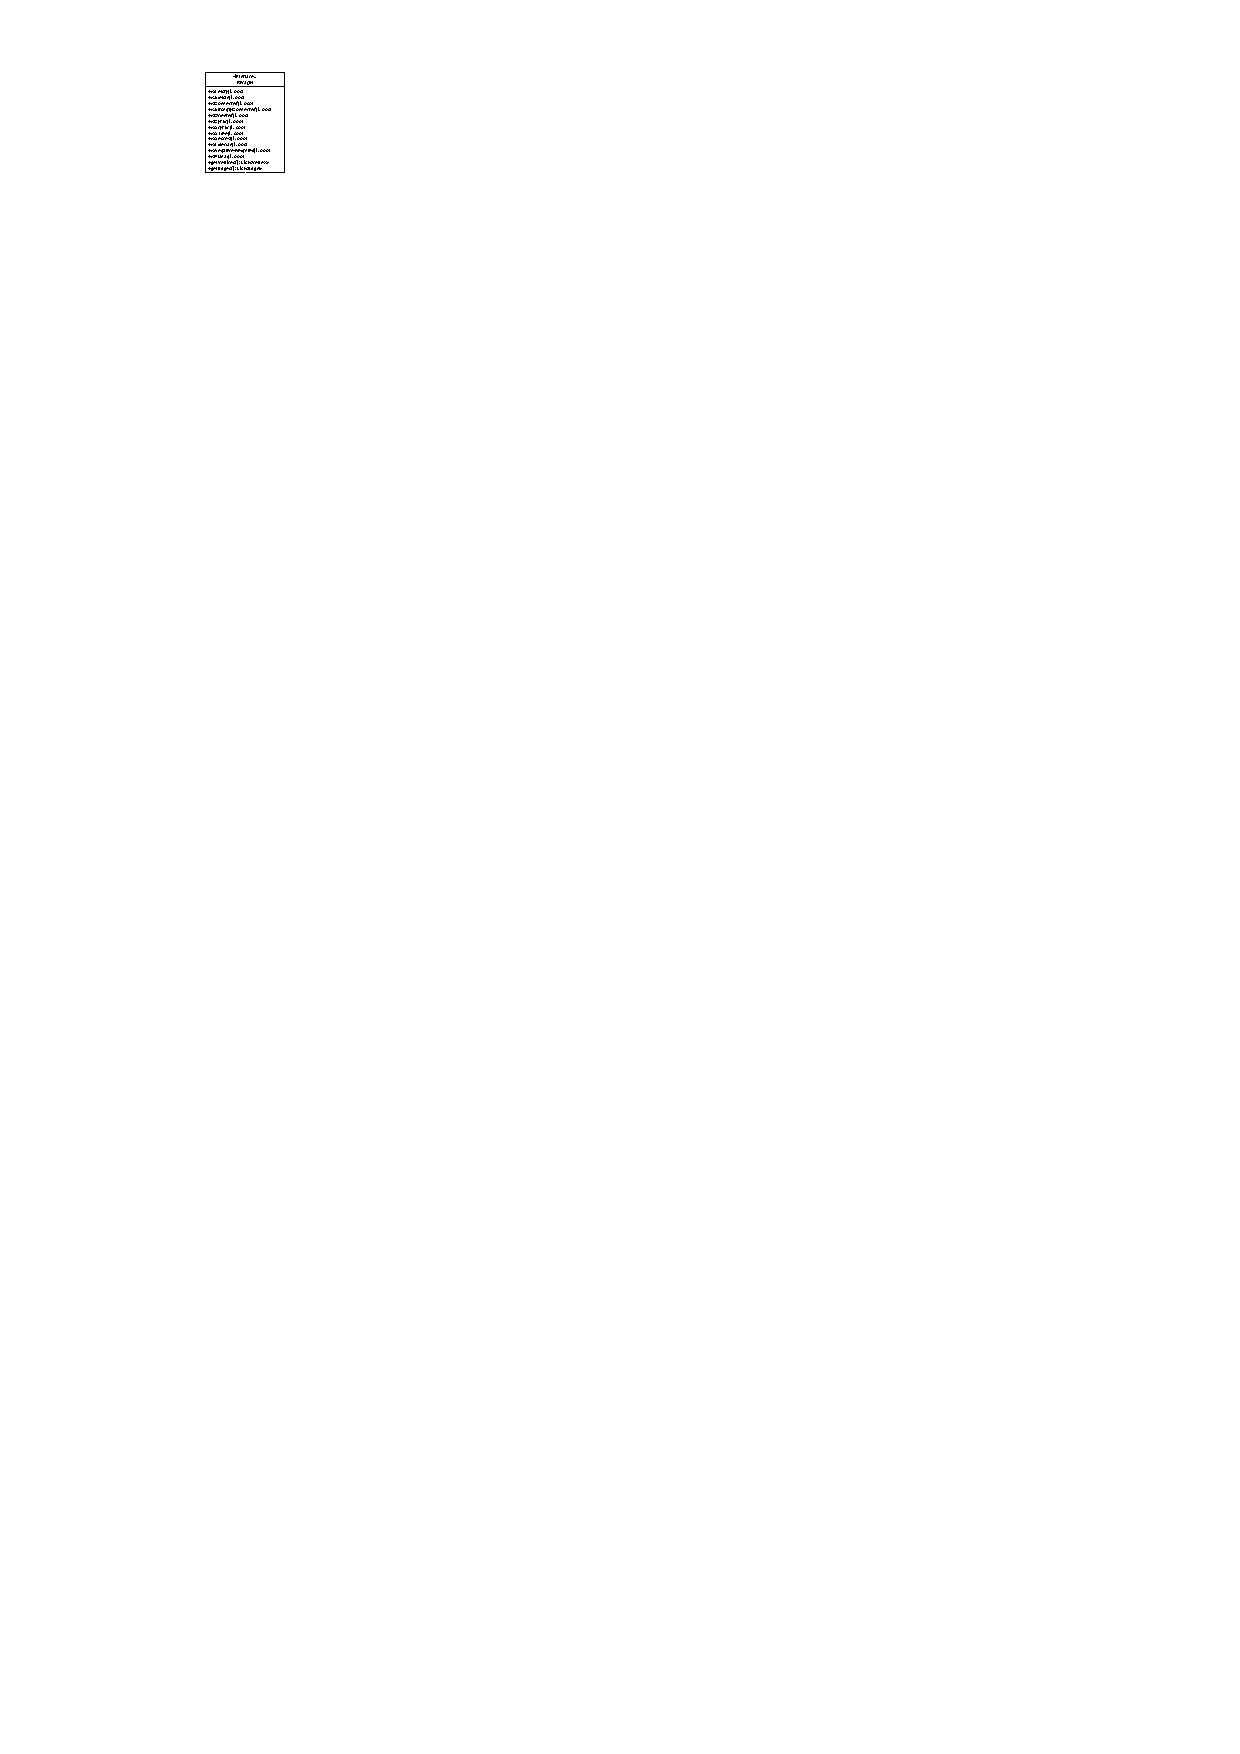
\includegraphics[scale=3.0]{Conception/igraph.pdf}
				\caption{Interface IGraph}
			\end{figure}
			
			\subsubsection{Structure de donnée}
			On peut distinguer deux approches principales pour représenter et stocker un graphe :
			\begin{enumerate}
				\item à l'aide de matrices
				\item ou à l'aide de listes (ou tableaux)
			\end{enumerate}	
			L'utilisation de matrices est prépondérante dans la modélisation mathématique de nombreux problèmes et l'étude de certaines propriétés d'un graphe. Elle permet des vérifications rapides pour la présence ou non d'arcs/arêtes, mais est relativement lente lorsqu'il s'agit de les parcourir.
			
			Quant aux listes, notamment les listes d'adjacence, l'itération des arcs/arêtes est rapide mais la vérification de leurs présence est lente. Les listes sont une version compacte de représenter les matrices car elles stockent uniquement les arêtes existantes. Le gain de place mémoire est donc plus avantageux tant que le graphe n'est pas complet.\\
			
			À ce stade, le choix de l'un ou l'autre présente alors ses avantages et désavantages. Une petite étude nous a permis d'orienter notre choix : \\
			
			Une première approche simple nous permet de déterminer qu'un graphe stocké sous forme de matrice occupera $n^2$ octets, où n est le nombre de sommet. Dans ce cas, un type char ferait amplement l'affaire pour représenter chaque case, car, en non-signé, on pourrait avoir jusqu'à 255 arcs/arêtes entre deux sommets.\\
			\begin{figure}[H]
				\centering
				\[
				\kbordermatrix{
					& v_1 & v_2 & v_3 & v_4 & v_5 \\
					v_1 & 0 & 2 & 4 & 1 & 1 \\
					v_2 & 0 & 0 & 0 & 0 & 1 \\
					v_3 & 1 & 0 & 0 & 0 & 1 \\
					v_4 & 0 & 3 & 0 & 0 & 1 \\
					v_5 & 1 & 1 & 0 & 3 & 0
				}
				\]
				\caption{Matrice d'adjacence de char}
			\end{figure}
			
			La seconde approche vise à réduire la taille mémoire de façon à n'avoir qu'un seul bit par case pour la présence ou non d'une arête. Cette approche économise huit fois plus de mémoire mais est inutilisable lorsqu'il y a plus de deux arêtes entre deux sommets.\\
			\begin{figure}[H]
				\centering
				\[
				\kbordermatrix{
					& v_1 & v_2 & v_3 & v_4 & v_5 \\
					v_1 & 0 & 1 & 1 & 1 & 1 \\
					v_2 & 0 & 0 & 0 & 0 & 1 \\
					v_3 & 1 & 0 & 0 & 0 & 1 \\
					v_4 & 0 & 0 & 0 & 0 & 1 \\
					v_5 & 1 & 1 & 0 & 0 & 0
				}
				\]
				\caption{Matrcide d'adjacence de bit}
			\end{figure}
			
			Ces deux premières approches ne permettent pas de stocker beaucoup d'informations concernant les Edge, c'est pourquoi nous nous tournons vers une troisième approche qui consiste à stocker des pointeurs de Edge (Edge = arc ou arête), ou nullptr lorsque l'arc/arête n'est pas présent. Pour pouvoir stocker plusieurs Edge, chaque case contient un pointeur vers une collection d'objets Edge.
			Cette troisième approche nécessite néanmoins 32 bits par case donc une taille mémoire de 4 $*$ $n^2$ octets.\\
			\begin{figure}[H]
				\centering
				\[
				\text{Mat}_{\varphi\text{ to }M} = \kbordermatrix{
					& v_1 & v_2 & v_3 & v_4 & v_5 \\
					v_1 & nullptr & *edges  & nullptr & *edges  & *edges   \\
					v_2 & nullptr & nullptr & nullptr & nullptr & nullptr  \\
					v_3 & *edges  & nullptr & nullptr & nullptr & *edges   \\
					v_4 & nullptr & nullptr & nullptr & nullptr & *nullptr \\
					v_5 & *edges  & *edges  & nullptr & nullptr & nullptr
				}
				\]
				\caption{Matrice d'adjacence de collection d'Edge}
			\end{figure}				
				
			
			Cependant, après avoir suivi le cours de GRE, nous nous sommes rendus compte qu'il était rare d'obtenir des graphes complets. La majorité des cas d'utilisation requièrent des graphes de faible densité, ce qui nous amène vers une quatrième approche : stocker les graphes sous forme de liste d'adjacence.\\
			
			Mis à part les aspects liés au gain de mémoire, les listes d'adjacences facilitent la plupart des opérations présentes dans nos algorithmes (discutés en section \textbf{\color{red}SECTION ALGOS}).
			Trouver tous les sommets adjacents à un certain sommet est aussi simple que lire la liste et prend un temps proportionnel au nombre de voisins. Avec une matrice, toute une ligne doit être lue, ce qui prend un temps beaucoup plus long égal au nombre de sommet présent dans l'entièreté du graphe.
			
			Cette quatrième et dernière approche est celle que nous avons choisie car elle est la plus adaptée à nos besoins. \textbf{Nos graphes sont donc stockés sous forme de liste d'adjacence}.
			
			\subsubsection{Détails d'implémentation de la structure}
			Dans cette partie, nous définissons comment la liste d'adjacence est implémentée. Il existe trois manières de représenter une telle liste :
			\begin{enumerate}
				\item Pour chaque sommet, lui associer un tableau des sommets adjacents. Il n'y a pas de représentation explicite des arcs/arêtes.
				\item Un tableau indexé par les numéros de sommet, où chaque case contient une simple liste chainée constituée des sommets adjacents, ou des arcs/arêtes adjacent(e)s.
				\item Une approche plus orientée objet consiste à avoir une variable d'instance pour chaque sommet, pointant vers une collection d'objet qui liste les arcs/arêtes voisin(e)s. À l'opposé, chaque arc/arête pointe vers ses deux sommets qui la compose. 
			\end{enumerate}
			La solution (1) ne permet pas de stocker d'informations sur les arcs/arêtes. La solution (2) le permet pour autant qu'on choisisse une liste d'Edge adjacents. Dans ce cas, on ne peut pas stocker d'information sur les sommets.\\
			
			Nous avons donc opté pour la solution (3). Un tableau de sommet, où chaque sommet possède une variable pointant vers une listes de pointeurs de Edge.\\
			À noter que pour un graphe non orienté, les Edge se répéteront à double et c'est précisément ce que nous voulons car nous souhaitons préserver la logique de la liste d'adjacence pour nos algorithmes.\\
			
			Voici un exemple de liste d'adjacence. *e$\{chiffre\}$ est un pointeur sur l'Edge $\{chiffre\}$. Les chiffres en marge à gauche sont les index des sommets.
			\begin{figure}[H]
				\centering
				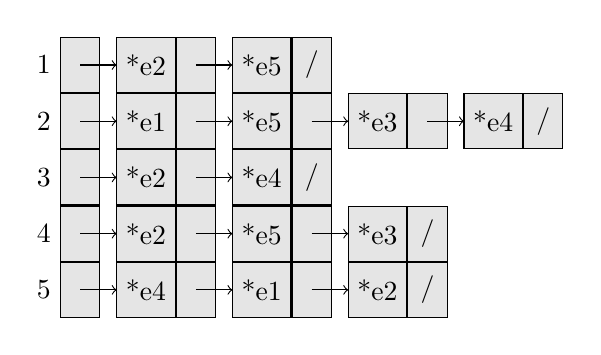
\begin{tikzpicture}
				\matrix (M) [matrix of nodes,
				column sep=0pt,
				row sep=0pt,
				nodes={draw,fill=gray!20,minimum width=.5cm,outer sep=0pt,minimum
					height=.7cm,anchor=center},
				column 1/.style={minimum height=.8cm}]{
					\mbox{} &[2mm] *e2 & \mbox{} &[2mm] *e5 & $/$  &[2mm]   &   &[2mm]   & \\
					\mbox{} & *e1 & \mbox{} & *e5 & \mbox{}  & *e3 &  \mbox{} & *e4 & $/$  \\
					\mbox{} & *e2 & \mbox{} & *e4 & $/$  &   &   &   & \\
					\mbox{} & *e2 & \mbox{} & *e5 & \mbox{}  & *e3 & $/$  &   & \\
					\mbox{} & *e4 & \mbox{} & *e1 & \mbox{}  & *e2 & $/$  &   & \\
				};
				\foreach \i in {1,2,3,4,5}{
					\path (M-\i-1) [late options={label=left:\i}];
					\draw[->] (M-\i-1.center)--(M-\i-2.west);
					\draw[->] (M-\i-3.center)--(M-\i-4.west);
				}
				\draw[->] (M-2-5.center)--(M-2-6.west);
				\draw[->] (M-4-5.center)--(M-4-6.west);
				\draw[->] (M-5-5.center)--(M-5-6.west);
				\draw[->] (M-2-7.center)--(M-2-8.west);
				\end{tikzpicture}
				\caption{Liste d'adjacence}
			\end{figure}
			Dans cet exemple:
			\begin{itemize}
				\item le sommet 1 possède deux Edge adjacents e2 et e5.
				\item le sommet 2 possède quatre Edge adjacents e1, e5, e3, e4.
				\item le sommet 3 possède deux Edge adjacents e3 et e4.
				\item etc.
			\end{itemize}
			
			
			
			\subsubsection{Création de graphes}
			Le patron de conception "fabrique" permet aux utilisateurs de créer un graphe à partir de toute structure représentative de graphe (matrice d'adjacence, liste de sommets et d'arcs, etc.).
			\begin{figure}[H]
				\centering
				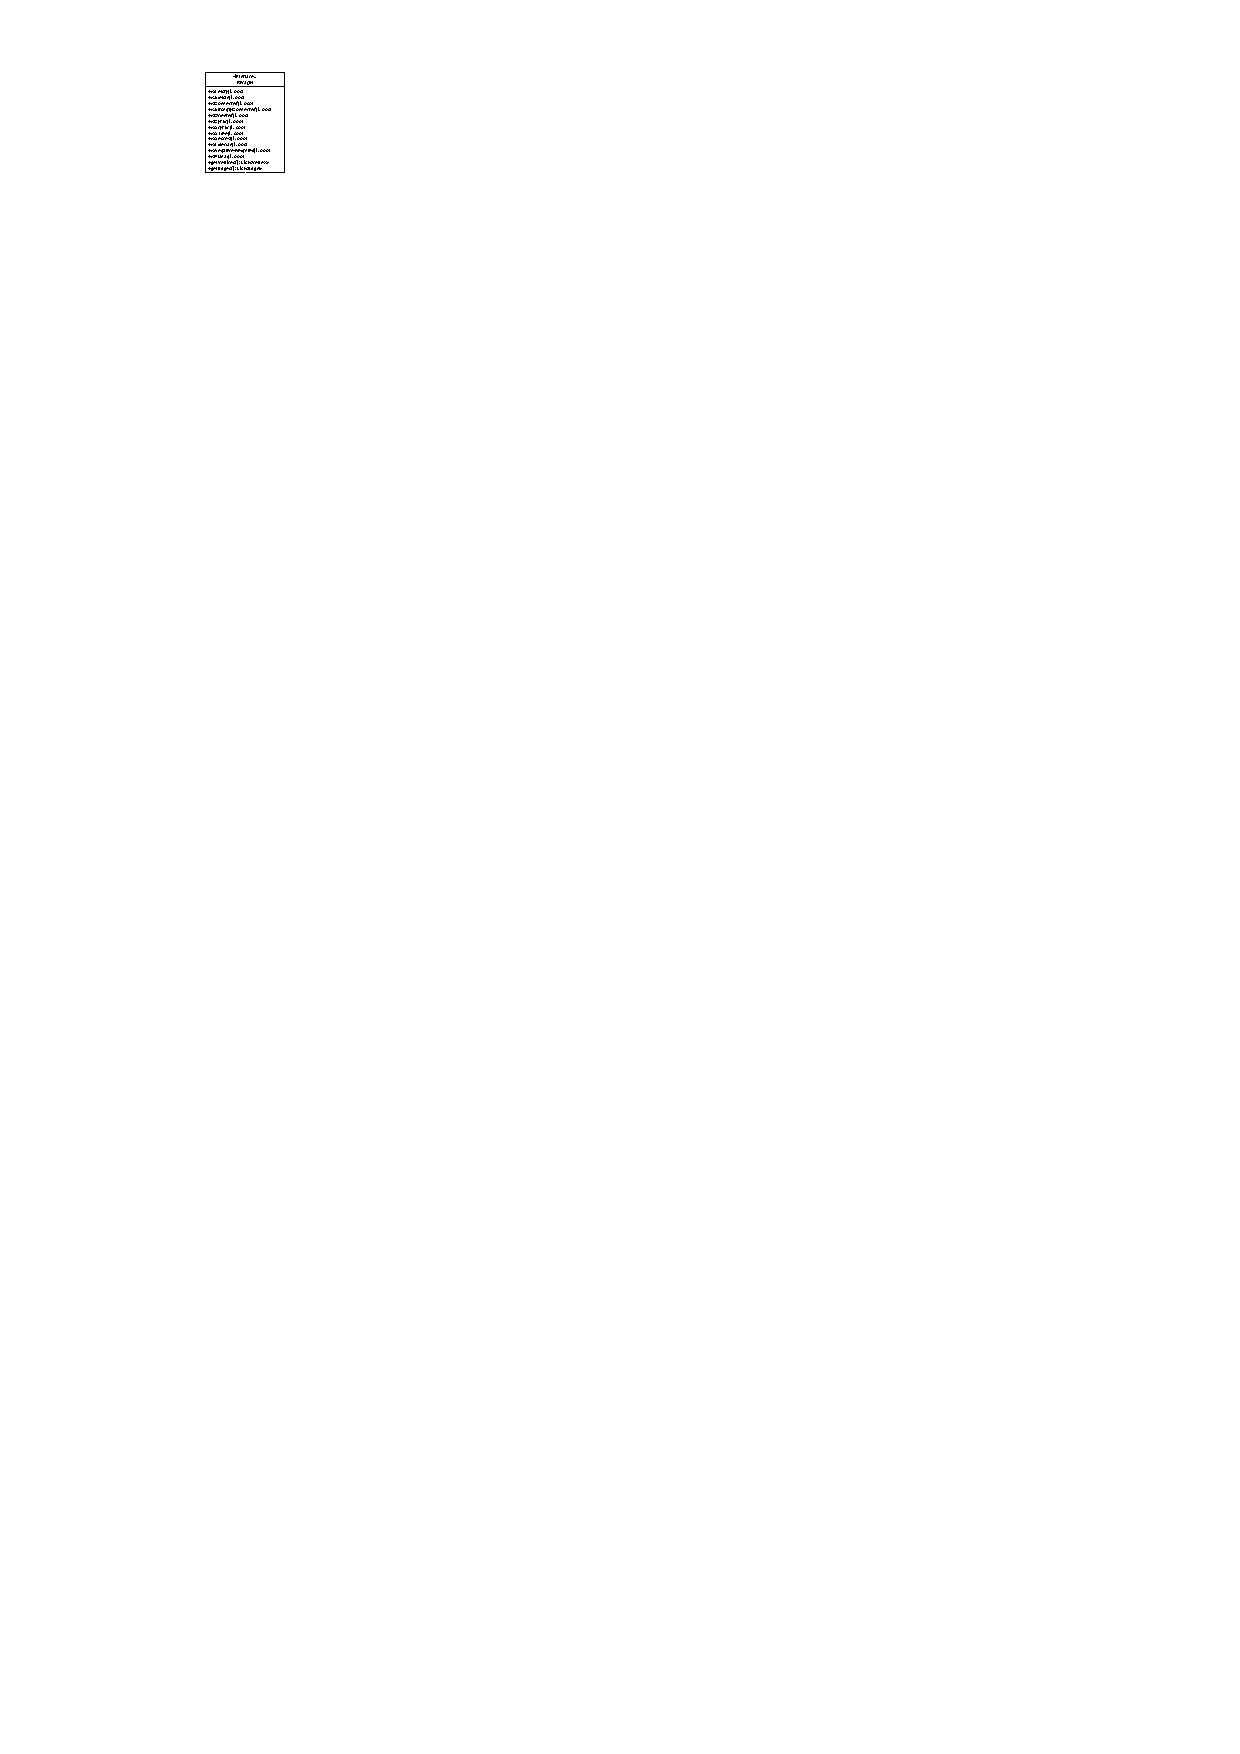
\includegraphics[scale=3.0]{Conception/igraph.pdf}
				\caption{Interface IGraph}
			\end{figure}
			
		
		\subsection{Algorithmes}
			\subsubsection{famille 1...}
		\subsection{blabla..}
	
	\section{Annexes}
	
		\subsection{Fonctions incluses}
			\label{subsec:annexes-fonctions-incluses}
			Cet annexe recense les fonctions incluses dans l'interpréteur et disponibles pour l'utilisateur de l'application. Les fonctions \textit{built-in} viennent de l'interpréteur directement, et les fonctions \textit{algo} proviennent de la couche sur les graphes et ses algorithmes.\\
			
			Note: les paramètres de type \texttt{T} indiquent qu'il existe une surcharge de la fonction pour chacun des types disponible dans le langage.
			
			\begin{figure}[H]
				\centering
				\begin{tabular}{lll}
					Prototype & Description & Origine\\
					\hline
					\texttt{String toString(T a)} & Retourne la représentation sous forme de chaîne de \texttt{a} & \textit{built-in}\\
					\texttt{} & & \textit{}\\
				\end{tabular}
			\end{figure}
	
	\begin{thebibliography}{9}
		\bibitem{qtStyle}
		Qt wiki, Qt coding style,\\ \url{https://wiki.qt.io/Qt_Coding_Style}
		
		\bibitem{vutbr.cz} 
		Faculty of Technology, Brno University of Technology, République tchèque,\\ \url{http://www.fit.vutbr.cz/study/courses/APR/public/ebnf.html}
		
		\bibitem{plantuml}
		PlantUML, Open-source tool that uses simple textual descriptions to draw UML diagrams,\\ \url{http://plantuml.com/}\\ \url{http://www.planttext.com/planttext}

		\bibitem{Graph data wikipedia.org}
		Graphs data structures,\\ \url{https://en.wikipedia.org/wiki/Adjacency_matrix#Data_structures}
	\end{thebibliography}			

\end{document}
